\documentclass[oneside,12pt]{Classes/aesm_edspia}
%\usepackage[latin1]{inputenc}
\usepackage[english,french]{babel}
\usepackage[T1]{fontenc}
\usepackage{amsmath}
\usepackage{lmodern}%font modern
\rmfamily
\DeclareFontShape{T1}{lmr}{bx}{sc}{<->ssub * cmr/bx/sc}{} %manque une police en lmodern
\usepackage{lettrine}
\usepackage{tabularx}
\usepackage{epsfig, floatflt, amssymb} 
\usepackage{wrapfig}%figure entour� de texte.
\usepackage{moreverb} %% pour le verbatim en boite
\usepackage{cases}%equations en systemes num�rot�s - soluce possible package : CASES
%\usepackage{slashbox} %% pour couper les colonnes des tableaux en diagonale 
%\usepackage{layout}
%\usepackage{showkeys} %% pour voir les labels
\usepackage{multirow} %% pour regrouper un texte sur plusieurs lignes dans une table
\usepackage{url} %% pour citer les url par \url
\usepackage[all]{xy} %% pour la barre au dessus des symboles
%\usepackage{shorttoc} %% pour plusieurs tables des mati�res par la commande \shorttableofcontents{Titre}{profondeur}.
\usepackage{textcomp} %% pour le symbol pour mille par \textperthousand et degr�s par \degres
\usepackage[right]{eurosym}
\usepackage{setspace} %interligne simple, double etc...
\usepackage{eurosans} %%pour le symbole \euro
\usepackage{epic,eepic}
\usepackage{soul}
%\usepackage{lineno}%num�roter les lignes 
\usepackage[nottoc]{tocbibind} % tables des figures, des matieres et autres dans la TOC
%\usepackage{palatino}
\usepackage{fancybox}
\usepackage[leftcaption]{sidecap}
%\usepackage[labelsep=endash, textfont={normalsize,onehalfspacing}, margin=5pt, format=hang, labelfont=bf]{caption}
\usepackage[labelsep=endash, textfont={footnotesize, singlespacing}, margin=10pt, format=plain, labelfont=bf]{caption}
\usepackage[Conny]{fncychap} %en tete chapitrage
\newcommand{\ie}{c.-\`a-d.~}
\hbadness=10000% pb d'overfull box r�gl�
\hfuzz=50pt
\pdfcompresslevel9 % pour compresser le pdf final au maximum
\pdfoptionpdfminorversion=5 % pour accept� les images PDF version 1.5 (ex: celles produites par Office 2007)
\def\underscore{\char`\_}
\makeatletter
\renewcommand{\thesection}{\arabic {section}}
\renewcommand{\SC@figure@vpos}{c}% centrer verticalement le caption avec le package sidecap...
\renewcommand{\fnum@figure}{\small\textbf{Figure~\thefigure}}
\renewcommand{\fnum@table}{\small\textbf{Tableau~\thetable}}
%\newcommand\figcaption{\def\@captype{figure}\caption}
%\newcommand\tabcaption{\def\@captype{table}\caption}
\makeatother
\usepackage{subfig}
\def\thechapter{\Roman{chapter}}
%\usepackage{chapterbib}

%%%%%%%%%%%%%%%%changement par moi
%\usepackage{xcolor}
%\usepackage{colorlinks=true,urlcolor=black}{hyperref}
\usepackage{multibib}
\usepackage{rotating}
\providecommand{\tabularnewline}{\\}
\usepackage{graphicx}
%\begin{maliste}
%\item
%\end{maliste}
\newenvironment{maliste}%
{ \begin{list}%
{$\bullet$}%
{\setlength{\labelwidth}{30pt}%
\setlength{\leftmargin}{45pt}%
\setlength{\itemsep}{\parsep}}}%
{ \end{list} }

%%
%%%%%%%%%%%%%%%
\newenvironment{lyxlist}[1]
{\begin{list}{}
{\settowidth{\labelwidth}{#1}
 \setlength{\leftmargin}{\labelwidth}
 \addtolength{\leftmargin}{\labelsep}
 \renewcommand{\makelabel}[1]{##1\hfil}}}
{\end{list}}
%%%%%%%%%%%%%%%%%%%%%%%%%%%%%%%%%%%%%%%%%%%
\begin{document}
%%%%%%%%%%%%%%%%%%%%%%%%%%%%%%%%%%%%%%%%%%%
\renewcommand\figurename{\small\textbf{Figure}} 

\addtocounter{page}{-1}%pour revenir � 0

%%  1ere de Couverture:
%\RapporteurA{M. xx xxxxx}{Professeur d'Universit�}{Rapporteur}
%\RapporteurB{M. xx xxxxx}{Directeur de Recherche au CNRS}{Rapporteur}
%\ExaminateurA{M. xx xxxxx}{Directeur de Recherche au CNRS}{Examinateur}
%\President{M. xx xxxxx}{Professeur d'Universit�}{Examinateur}         
%\ExaminateurB{M. xx xxxxx}{Charg� de Recherche au CNRS}{Examinateur}


%\makethese %% cr�e la couverture.

\onehalfspacing
%\renewcommand\baselinestretch{1.2}
%\baselineskip=18pt plus 1pt

% une page blanche (deuxi�me de couverture)

%\newpage\thispagestyle{empty}\addtocounter{page}{-1}
%\null\newpage\thispagestyle{empty}

%\newpage\thispagestyle{empty}
%~\newpage\thispagestyle{empty}

%profondeur dans la table des mati�res et de la num�rotation des sections
\setcounter{secnumdepth}{3}
\setcounter{tocdepth}{3}


\frontmatter
%\pagestyle{fancy}
%\fancyhf{}
\chapter*{Remerciement}
%=================================================================%

\textbf{\Huge A}u terme de ce travail, nous avons le plaisir d'exprimer nos vifs
et sinc�res remerciements � notre encadreur : M. Sidhom Walid, pour
son appui contenu durant toute la p�riode du projet. En effet, ses
conseils ont �t� pour nous des ressources essentielles � la r�alisation
de ce travail.
\\

Nos remerciements s'adressent aussi aux membres du jury qui ont accept�
de juger ce modeste travail.
\\

Nos mains se l�vent �galement vers nos amis de la classe G�nie Informatique
21, pour leurs critiques constructives � l\textquoteright{}�gard de
notre petite m�moire et pour leur encouragement durant les deux ann�es
qu\textquoteright{}on a pass�es ensemble.
\\ 

Enfin, nous tenons � exprimer nos sentiments les plus respectueux
responsables de l'Acad�mie Militaire, sp�cialement le commandement
de l'Acad�mie Militaire, les officiers du groupement �l�ve, le personnel
de d�partement service informatique et tous ceux qui nous ont encourag�
et soutenu au long de ce projet.         

%\fancyhead[R]{Remerciements}
%\fancyhead[RO]{\bfseries\rightmark}
%\fancyhead[LE]{\bfseries\leftmark}
%\fancyfoot[R]{\thepage}
%\fancyfoot[LE]{\thepage}
%\renewcommand{\headrulewidth}{0.5pt}
%\renewcommand{\footrulewidth}{0pt}
%\renewcommand{\chaptermark}[1]{\markboth{\MakeUppercase{\chaptername~\thechapter. #1 }}{}}
%\renewcommand{\sectionmark}[1]{\markright{\thechapter.\thesection~ #1}}

%\printnomenclaturey
\pagestyle{fancy}
\fancyhf{}
\fancyhead[R]{Table des mati�res}
%\fancyhead[RO]{\bfseries\rightmark}
%\fancyhead[LE]{\bfseries\leftmark}
\fancyfoot[R]{\thepage}
%\fancyfoot[LE]{\thepage}
\renewcommand{\headrulewidth}{0.5pt}
\renewcommand{\footrulewidth}{0pt}
%\renewcommand{\chaptermark}[1]{\markboth{\MakeUppercase{\chaptername~\thechapter. #1 }}{}}
%\renewcommand{\sectionmark}[1]{\markright{\thechapter.\thesection~ #1}}
\tableofcontents
%%%%%%%%%%%%%%
\listoffigures
\pagestyle{fancy}
\fancyhf{}
\fancyhead[R]{Table des figures}
%\fancyhead[RO]{\bfseries\rightmark}
%\fancyhead[LE]{\bfseries\leftmark}
\fancyfoot[R]{\thepage}
%\fancyfoot[LE]{\thepage}
\renewcommand{\headrulewidth}{0.5pt}
\renewcommand{\footrulewidth}{0pt}
%\renewcommand{\chaptermark}[1]{\markboth{\MakeUppercase{\chaptername~\thechapter. #1 }}{}}
%\renewcommand{\sectionmark}[1]{\markright{\thechapter.\thesection~ #1}}
%%%%%%%%%%%%%

%%%%%%%%%%%%%%%%%%
%%%%%%%%%%%%%%%%%%
\listoftables
%%%%%%%%%%%%%
\pagestyle{fancy}
\fancyhf{}
\fancyhead[R]{Convention}
%\fancyhead[RO]{\bfseries\rightmark}
%\fancyhead[LE]{\bfseries\leftmark}
\fancyfoot[R]{\thepage}
%\fancyfoot[LE]{\thepage}
\renewcommand{\headrulewidth}{0.5pt}
\renewcommand{\footrulewidth}{0pt}
%\renewcommand{\chaptermark}[1]{\markboth{\MakeUppercase{\chaptername~\thechapter. #1 }}{}}
%\renewcommand{\sectionmark}[1]{\markright{\thechapter.\thesection~ #1}}
%%%%%%%%%%%%%
\section*{Convention}
Les diff�rentes typographies utilis�es dans ce document sont les suivantes :
\begin{maliste}
 \item une typographie ordinaire pour le texte, trois syles : romain (ordinaire), \textit{italique}, et \textbf{gras} (ou \textbf{\textit{italiquegras}}),
 \item \textbf{une mise en gras} pour les termes figurant dans le glossaire (Annexe A).
\end{maliste}

                                      
\mainmatter
\pagestyle{fancy}
\fancyhf{}
\fancyhead[R]{Introduction g�n�rale}
%\fancyhead[RO]{\bfseries\rightmark}
%\fancyhead[LE]{\bfseries\leftmark}
\fancyfoot[R]{\thepage}
%\fancyfoot[LE]{\thepage}
\renewcommand{\headrulewidth}{0.5pt}
\renewcommand{\footrulewidth}{0pt}
%\renewcommand{\chaptermark}[1]{\markboth{\MakeUppercase{\chaptername~\thechapter. #1 }}{}}
%\renewcommand{\sectionmark}[1]{\markright{\thechapter.\thesection~ #1}}
\chapter*{Introduction g�n�rale}

\addcontentsline{toc}{chapter}{Introduction g�n�rale}
%==================================================================================================%


De nos jours, l'informatique est devenue une pi�ce maitresse dans   l'acquisition et le traitement de l'information sous toutes ses formes. De ce fait les syst�mes informatiques sont omnipr�sents.
\\
  
Malheureusement, dans notre soci�t� ce domaine attire de plus en plus des personnes malintentionn�es qui tentent de compromettre leur int�grit�, confidentialit� ou disponibilit�. En effet, les entreprises et les particuliers se voient donc confront�s de fa�on quotidienne � des vers, des virus, des attaques de tout type de tentatives d'intrusions. La s�curit� est plus que jamais une probl�matique d'actualit� et nous pouvons facilement le constater en
parcourant les journaux de la presse sp�cialis�e.
\\
  
Un moyen rapide de conna�tre l'�tendue de la fragilit� d'un environnement, vis � vis
des attaques diverses et vari�es, est d'effectuer des tests d'intrusions qui permettent d'avoir
une liste de failles de vuln�rabilit�s potentielles.
Dans ce cadre se situe notre projet, intitul� << Etude et mise en place d'un environnement d'analyse r�seau et de test d'intrusion >>.
\\
  
Ce document est le rapport des travaux entrepris durant ce projet de fin d'ann�e, r�alis� au sein de l'Acad�mie Militaire.Il a une �tude bibliographique de la s�curit�: L'introduction est suivie d'un premier chapitre consacr� � l'introduction de la s�curit� et ses objectifs et aux divers types d'attaques. Par la suite, le second chapitre abordera l'analyse r�seau et ses diff�rents outils. Le troisi�me chapitre pr�sentera les tests d'intrusion. Lors du quatri�me et dernier chapitre, nous pr�senterons les diff�rentes �tapes de r�alisation de nos tests, avant d'aborder la conclusion g�n�rale.


\chapter{Introduction � la s�curit� informatique}
\graphicspath{{Chapitre1/figures/}}
%==============================================================================
\pagestyle{fancy}
\fancyhf{}
\fancyhead[R]{\bfseries\leftmark}
%\fancyhead[LE]{}
\fancyfoot[R]{\thepage}
%\fancyfoot[LE]{\thepage}
\renewcommand{\headrulewidth}{0.5pt}
\renewcommand{\footrulewidth}{0pt}
\renewcommand{\chaptermark}[1]{\markboth{\MakeUppercase{\chaptername~\thechapter. #1 }}{}}
\renewcommand{\sectionmark}[1]{\markright{\thechapter.\thesection~ #1}}
%==============================================================================
\section{D�finition}




La s�curit� informatique est l'ensemble des moyens mis en \oe uvre
pour minimiser la vuln�rabilit� d'un syst�me contre des menaces accidentelles
ou inaccidentelles. Conna�tre les dangers auxquels il convient de parer, et conna�tre
les moyens de se pr�munir contre eux. La s�curit� exige de se montrer
syst�matique, mais elle implique aussi un effort de coordination,
de technologie, d'information, de discussion, de comparaison et de
contr�le. 


\section{Objectifs g�n�raux de la s�curit� informatique}

La s�curit� informatique\cite{1}, d'une mani�re g�n�rale, consiste � assurer
que les ressources mat�rielles ou logicielles d'une organisation sont
uniquement utilis�es dans le cadre pr�vu. 
\\

La s�curit� informatique vise g�n�ralement cinq principaux objectifs :



\subsection*{L'int�grit�}

la v�rification de l'int�grit� des donn�es consiste � d�terminer si les donn�es
n'ont pas �t� modifi�es durant la communication (de mani�re fortuite
ou intentionnelle). 

\subsection*{La confidentialit�}

La confidentialit� consiste � rendre l'information inintelligible(ind�chiffrable)
� d'autres personnes que les seuls acteurs de la transaction. 


\subsection*{La disponibilit�}

Son objectif est de garantir l'acc�s � un service
ou � des ressources. 


\subsection*{La non-r�pudiation}

La non-r�pudiation de l'information est la garantie qu'aucun des correspondants
ne pourra nier la transaction.


\subsection*{L'authentification}

L'authentification consiste � assurer l'identit� d'un utilisateur,
c'est-�-dire de garantir � chacun des correspondants que son partenaire
est bien celui qu'il croit �tre. Un contr�le d'acc�s peut permettre
(par exemple par le moyen d'un mot de passe qui devra �tre crypt�)
l'acc�s � des ressources uniquement aux personnes autoris�es. 



\section{Vuln�rabilit�}


\subsection{D�finition }
Dans le domaine de la s�curit� informatique\cite{2}, une vuln�rabilit� est une faiblesse dans un syst�me informatique permettant � un attaquant de porter atteinte � l'int�grit� de ce syst�me, c'est-�-dire � son fonctionnement normal, � la confidentialit� et l'int�grit� des donn�es qu'il contient. On parle aussi de faille de s�curit� informatique.


\subsection{Causes}

La cause des vuln�rabilit�s informatiques est souvent la n�gligence ou l'inexp�rimentation d'un programmeur. Une vuln�rabilit� permet g�n�ralement � l'attaquant de tromper l'application, par exemple en d�passant les v�rifications de contr�le d'acc�s ou en ex�cutant des commandes sur le syst�me h�bergeant l'application.

Exemples de vuln�rabilit�s
\begin{maliste}
\item D�passement de tampon
\item Injection \textbf{SQL}
\item Cross site scripting
\end{maliste}

Quelques vuln�rabilit�s surviennent lorsque l'entr�e d'un utilisateur n'est pas contr�l�e, permettant l'ex�cution de commandes ou de requ�tes \textbf{SQL} (connues sous le nom d'injection \textbf{SQL}). D'autres proviennent d'erreurs d'un programmeur lors de la v�rification des buffers de donn�es (qui peuvent alors �tre d�pass�s), causant ainsi une corruption de la pile m�moire (et ainsi permettre l'ex�cution de code fourni par l'attaquant).

\subsection{Identification et correction des vuln�rabilit�s}

Il existe de nombreux outils qui peuvent faciliter la d�couverte de vuln�rabilit�s sur un syst�me information, certains permettant leur suppression. Mais, bien que ces outils puissent fournir � un auditeur une bonne vision d'ensemble des vuln�rabilit�s potentiellement pr�sentes, ils ne peuvent pas remplacer le jugement humain. Se reposer uniquement sur des scanners automatiques de vuln�rabilit� rapportera de nombreux faux positifs et une vue limit�e des probl�mes pr�sents dans le syst�me.

Exemples de ces outils
\begin{description}
\item [{Nessus, OpenVAS}] scanners de vuln�rabilit�s
\item [{Wapiti, Nikto}] analyseurs de Site Web
\item [{Absynthe, SQLNinja, SQLInject}] analyseurs de Base de donn�es 
\end{description}



\section{Les types d'attaques}

les attaques\cite{Cederic}, qui visent ces failles, (voir fig \ref{chap1}) peuvent �tre � la fois tr�s vari�es
et tr�s dangereuses. C\textquoteright{}est pourquoi nous allons dans
tout d\textquoteright{}abord analyser ce que nous appellerons  << l\textquoteright{}anatomie
d\textquoteright{}une attaque >> , ensuite, nous caract�riserons
ces attaques et observerons leur d�roulement.

\begin{figure}[!ht]
  \centering
\includegraphics[scale=1]{shem1.png}
\caption{\label{chap1}Typologie des faiblesses de s�curit�.}
\end{figure}



\subsection{Anatomie d\textquoteright{}une attaque}

Fr�quemment appel�s << les 5 P >> dans la litt�rature, ces cinq verbes
anglophones constituent le squelette de toute attaque informatique
: Probe, Penetrate, Persist, Propagate, Paralyze.
\begin{maliste}

\item \underbar{Probe} (approfondir): consiste en la collecte d\textquoteright{}informations
par le biais d\textquoteright{}outils
\item \underbar{Penetrate}(p�n�trer) : utilisation des informations r�colt�es pour
p�n�trer un r�seau.
\item \underbar{Persist}(persister) : cr�ation d\textquoteright{}un compte avec des
droits de super utilisateur pour pouvoir se r�infiltrer ult�rieurement.
\item \underbar{Propagate}(propager) : cette �tape consiste � observer ce qui est
accessible et disponible sur le r�seau local.
\item \underbar{Paralyze}(paralyser) : cette �tape peut consister en plusieurs actions.
Le pirate peut utiliser le serveur pour mener une attaque sur une
autre machine, d�truire des donn�es ou encore endommager le syst�me
d\textquoteright{}exploitation dans le but de planter le serveur.
\end{maliste}
Apr�s ces cinq �tapes, le pirate peut �ventuellement tenter d\textquoteright{}effacer
ses traces, bien que cela ne soit rarement utile.


\subsection{Les attaques r�seaux}

Ils se basent principalement sur des failles li�es aux protocoles
ou � leur impl�mentation. Observons quelques attaques bien connues.


\subsubsection{Les techniques de scan}

Le but des scans est de d�terminer quels sont les ports ouverts, et
donc en d�duire les services qui sont ex�cut�s sur la machine cible
(ex : port 80/TCP pour un service HTTP). Par cons�quent, la plupart
des attaques sont pr�c�d�es par un scan de ports lors de la phase
Probe.


\subsubsection{Les attaques d\textquoteright{}acc�s}

Une attaque d\textquoteright{}acc�s est une tentative d\textquoteright{}acc�s
� l\textquoteright{}information par une personne non autoris�e. Ce
type d\textquoteright{}attaque concerne la confidentialit� de l\textquoteright{}information.


\subsubsection*{\textit{Le sniffing}}

Cette attaque est utilis�e par les pirates informatiques pour obtenir
des mots de passe. Gr�ce � un logiciel appel� renifleur de paquets
(sniffer), on peut intercepter toutes les paquets qui circulent sur
un r�seau m�me ceux qui ne nous sont pas destin�s. Cette technologie
n\textquoteright{}est pas forcement ill�gale car elle permet aussi
de d�tecter des failles sur un syst�me.


\subsubsection*{\textit{Les chevaux de Troie et Porte d�rob�e}}

Les chevaux de Troie sont des programmes informatiques cach�s dans
d\textquoteright{}autres programmes. Leur but est de cr�er une porte
d�rob�e (backdoor) pour qu\textquoteright{}un pirate informatique
puisse ensuite acc�der facilement l\textquoteright{}ordinateur ou
le r�seau informatique. 

Il existe diff�rents types de portes d�rob�es :
\begin{maliste}

\item Cr�ation d\textquoteright{}un nouveau compte administrateur avec un
mot de passe choisi par le pirate.
\item Cr�ation de compte ftp
\item Modification des r�gles du pare-feu pour qu\textquoteright{}il accepte
des connections externes.
\end{maliste}
Dans tous les cas, l\textquoteright{}administrateur pert le contr�le
total du syst�me informatique. Il peut voler des mots de passe, copier
des donn�es, ex�cuter des actions nuisibles.


\subsubsection*{\textit{L\textquoteright{}ing�nierie sociale}}

C\textquoteright{}est une m�thode pour obtenir des informations sur
un syst�me ou des mots de passe. Elle consiste surtout � se faire
passer pour quelqu\textquoteright{}un que l\textquoteright{}on est
pas (en g�n�ral un des administrateurs du serveur que l\textquoteright{}on
veut pirater) et de demander des informations personnelles (login,
mots de passe, acc�s, num�ros, donn�es\ldots{}) en inventant un quelconque
motif (plantage du r�seau, modification de celui-ci\ldots{}). 


\subsubsection*{\textit{Le craquage de mots de passe}}

Le craquage consiste � faire de nombreux essais jusqu\textquoteright{}�
trouver le bon mot de passe. Il existe deux grandes m�thodes :
\begin{maliste}

\item \textbf{L\textquoteright{}utilisation de dictionnaires :} le mot test�
est pris dans une liste pr�d�finie contenant les mots de passe les
plus courants. Les dictionnaires actuels contiennent dans les 50 000
mots et sont capables de faire une grande partie des variantes.
\item \textbf{La m�thode brute :} toutes les possibilit�s sont faites dans
l\textquoteright{}ordre jusqu\textquoteright{}� trouver la bonne solution.
\end{maliste}

\subsubsection{Les attaques par saturation (d�ni de service)}

Les attaques par saturation sont des attaques informatiques qui consiste
� envoyer des milliers de messages depuis des dizaines d'ordinateurs,
dans le but de submerger les serveurs d'une soci�t�, de paralyser
pendant plusieurs heures son site Web et d'en bloquer ainsi l'acc�s
aux internautes. Il existe diff�rente attaque par saturation : 


\subsubsection*{\textit{Le flooding }}

Il consiste � envoyer � une machine de nombreux paquets IP de grosse
taille. La machine cible ne pourra donc pas traiter tous les paquets
et finira par se d�connecter du r�seau.


\subsubsection*{\textit{Le smurf }}

Il s\textquoteright{}appuie sur le ping et les serveurs de broadcast
. On falsifie d\textquoteright{}abord son adresse IP pour se faire
passer pour la machine cible. On envoie alors un ping sur un serveur
de broadcast. Il le fera suivre � toutes les machines qui sont connect�es
qui renverront chacune un << pong >>
au serveur qui fera suivre � la machine cible. Celle-ci sera alors
inond�e sous les paquets et finira par se d�connecter.


\subsubsection*{\textit{Le d�bordement de tampon }}

Il se base sur une faille du protocole IP. On envoie � la machine
cible des donn�es d\textquoteright{}une taille sup�rieure � la capacit�
d\textquoteright{}un paquet. Celui-ci sera alors fractionn� pour l\textquoteright{}envoi
et rassembl� par la machine cible. A ce moment, il y aura d�bordement
des variables internes.


\subsubsection{Les attaques de r�pudiation}

La r�pudiation est une attaque contre la responsabilit�. Autrement
dit, la r�pudiation consiste � tenter de donner de fausses informations
ou de nier qu\textquoteright{}un �v�nement ou une transaction se soient
r�ellement pass�. Exemples de ces attaques :
\begin{maliste}

\item \textbf{LeARPspoofing} : consiste � se faire passer pour une autre
machine en falsifiant son adresse MAC. 
\item \textbf{LeIPspoofing} : consiste � se faire passer pour une autre
machine en falsifiant son adresse IP. 
\end{maliste}




\section{Conclusion}

De plus en plus la s�curit� contre les attaques distantes se renforce, notamment par
le biais d\textquoteright{}�quipements r�seaux plus puissants (comme
des firewalls plus intelligents), mais les attaques locales restent
encore fort efficaces.
 



\setcounter{chapter}{1}
\chapter{Analyse du r�seau}
\graphicspath{{Chapitre2/figures/}}

%==================================================================================================%
\section{Introduction}

Un << analyseur r�seau >>\cite{3} (appel� �galement analyseur de trames ou en
anglais \textit{sniffer}, traduisez << renifleur >>) est un dispositif
permettant d' �couter le trafic d'un r�seau, c'est-�-dire de capturer
les informations qui y circulent. 

En effet, dans un r�seau non commut�, les donn�es sont envoy�es �
toutes les machines du r�seau. Toutefois, dans une utilisation normale
les machines ignorent les paquets qui ne leur sont pas destin�s. Ainsi,
en utilisant l'interface r�seau dans un mode sp�cifique (appel� g�n�ralement
\textbf{mode promiscuous}) il est possible d'�couter tout le trafic
passant par un adaptateur r�seau (une carte r�seau ethernet, une carte
r�seau sans fil, etc.).
\section{D�finition}




\subsection{Utilisation du sniffer}

Un sniffer est un outil permettant d'�tudier le trafic
d'un r�seau. Il sert g�n�ralement aux administrateurs pour diagnostiquer
les probl�mes sur leur r�seau ainsi que pour conna�tre le trafic qui
y circule. Ainsi les d�tecteurs d'intrusion (\textbf{IDS}, pour intrusion
detection system) sont bas�s sur un sniffeur pour la capture des trames,
et utilisent une base de donn�es de r�gles pour d�tecter des
trames suspectes. 
 le sniffer peut aussi servir � une personne malveillante ayant un acc�s physique
au r�seau pour collecter des informations. Ce risque est encore plus
important sur les r�seaux sans fils car il est difficile de confiner
les ondes hertziennes dans un p�rim�tre d�limit�, si bien que des
personnes malveillantes peuvent �couter le trafic en �tant simplement
dans le voisinage. 


\subsection{Technique de fonctionnement}

Pour pouvoir �couter tout le trafic sur une interface r�seau, celle-ci
doit �tre configur�e dans un mode sp�cifique, le << \textbf{mode promiscuous}
>>. Ce mode permet d'�couter tous les paquets passant par l'interface,
alors que dans le mode normal, le mat�riel servant d'interface r�seau
�limine les paquets n'�tant pas � destination de l'h�te. 

La grande majorit� des protocoles Internet font transiter les informations
en clair, c'est-�-dire de mani�re non chiffr�e. Ainsi, lorsqu'un utilisateur
du r�seau consulte sa messagerie via le protocole \textbf{POP} ou
\textbf{IMAP}, ou bien surfe sur internet sur des sites dont l'adresse
ne commence pas par \textbf{HTTPS}, toutes les informations envoy�es
ou re�ues peuvent �tre intercept�es. C'est comme cela que des sniffers
sp�cifiques ont �t� mis au point par des pirates afin de r�cup�rer
les mots de passe circulant dans le flux r�seau. 

Le packet sniffer d�compose ces messages et les rassemble, ainsi les
informations peuvent �tre analys�es � des fins frauduleuses (d�tecter
des logins, des mots de passe, des emails), analyser un probl�me r�seau,
superviser un trafic ou encore faire de la \textbf{r�tro-ing�nierie}.



\section{Outils d'analyse r�seau}


\subsection{Wireshark}
Wireshark\cite{4} (connu comme Ethreal jusqu'� une discussion de la marque en �t� 2006) est un analyseur libre du protocole du r�seau pour Unix et Windows. Il nous permet d'examiner des donn�es d'un r�seau en direct ou d'un dossier de la capture sur disque. 
On conserve les donn�es de la capture interactivement, en creusant en bas dans seulement l'�gal de d�tail du paquet qu'on a besoin.
 
 Wireshark a des plusieurs traits puissants, y compris une langue du filtre de l'exposition riche et la capacit� de regarder le ruisseau reconstruit d'une session \textbf{TCP}. Il supporte aussi des centaines de protocoles et types de m�dia. 
Mais cet Ethereal a souffert de douzaines de  trous de  s�curit� exploitables de fa�on distante, donc il faut  �tre � jour et prudent de le faire tourner sur les r�seaux hostiles (tel que conf�rences de la s�curit�). 

\subsection{Tcpdump}
Tcpdump est le renifleur  classique  de l'\textbf{IP} qui �tait utilis� avant qu'Ethreal (Wireshark) est venu sur la sc�ne, et une majorit� continu � l'utiliser fr�quemment. Il ne peut pas avoir les  cloches et les sifflements  comme Wireshark ,  mais il travail bien  et avec moins de trous de  s�curit�.

 Il exige aussi moins de ressources du syst�me. Pendant qu'il ne re�oit pas souvent de nouveaux traits, il est maintenu active pour arrange des insectes et des probl�mes de la transferabilit�. Il y a une version  Windows s�par� nomm� WinDump.  


\subsection{Ettercap }
C'est un renifleur\cite{4} du r�seau terminal-bas� pour les r�seaux Ethernet \textbf{LAN}. Il supporte des examinateurs active  et passive de beaucoup de protocoles (m�me chiffr�s, comme \textbf{ssh} et \textbf{http}).
Une injection des donn�es dans un rapport peut �tre �tablie m�me  un filtrage  rapide est aussi possible, en gardant le rapport synchronis�. Beaucoup de modes reniflant ont �t� rendues effectif pour vous donner  une suite reniflant puissante et compl�te. Il a la capacit� de v�rifier si vous �tes dans un \textbf{LAN} switcher ou pas, et utilise  des empreintes digitales du Syst�me d'exploitation (actif ou passif) pour nous faire savoir la g�om�trie du \textbf{LAN}.


\subsection{Dsniff}
C'est � la fois une suite d'utilitaire\cite{4} et un utilitaire lui-m�me d'audit r�seau permettant ais�ment de sniffer les passwords circulants en clair, dans des protocoles non s�curis�s. 

Ainsi, Il d�tecte automatiquement les protocoles d'application, en capturant seulement les donn�es int�ressantes (Des mots clefs : pass, user,...). Elles concernent les sessions \textbf{FTP, telnet, SMTP, HTTP, POP, NNTP, IMAP, SNMP, LDAP, rlogin, RIP, OSPF, PPTP, AIM, IRC,...} 
Chacun de ses programmes a un but pr�cis (capture de mail, de fichier, d'url...). 

\subsection{SoftPerfect Analyser}
C'est est un outil avanc�, professionnel pour analyser, en d�pannant, en maintenant et dirigeant des r�seaux locaux et des rapports Internet.
 
 Il capture les donn�es qui passent � travers la carte Ethernet du r�seau, analyse ces donn�es puis le repr�sente dans une forme lisible. Il est un outil utile pour un administrateurs du r�seau, sp�cialistes de la s�curit�, promoteurs de l'application du r�seau et n'importe qui  a besoin d'une image compl�te de la circulation qui traverse leur rapport du r�seau ou segment d'un r�seau de r�gion local.


\subsection{Kismet}
 Kismet\cite{4} est un sniffer et un d�tecteur d'intrusion. Il fonctionne avec toutes les cartes supportant le monitoring (\textbf{rfmon}) et peut sniffer le trafic 802.11b, 802.11a, et 802.11g. Il est compos� d'un serveur et d'un client (par d�faut l'acc�s est restreint � l'adresse local) ce qui permet � plusieurs utilisateurs de voir un seul serveur Kismet simultan�ment. 
il peut d�tecter automatiquement les bloques IP du r�seau en reniflant TCP, UDP, ARP et paquets DHCP, circulant dans le r�seau estim�.

\section{Synth�se comparative}
\subsection{Tableau comparatif des outils}
Nous allons dans cette partie essayer de nous chercher � faire une comparaison entre ces diff�rents outils d'analyse r�seau, c'est � dire renseigner tous les crit�res de comparaison pour l'ensemble des produits choisis, de fa�on superficielle. Le but de notre �tude est de trouver l'outil le mieux adaptable � notre test qu'on va le r�aliser dans la partie R�alisation (chapitre 4). En effet, les r�sultats de comparaison nous ont men� � faire le tableau tab \ref{tabcomp}.
\begin{table}
\begin{center}



\begin{sideways}
\begin{tabular}{|c|c|c|c|c|c|c|c|c|}
\hline 
\multicolumn{2}{|c|}{\textbf{\textit{Crit�res}}} & \textbf{\footnotesize Wireshark} & \textbf{\footnotesize Tcpdump} & \textbf{\footnotesize Cain and Abel } & \textbf{\footnotesize Ettercap} & \textbf{\footnotesize Dsniff} & \textbf{\footnotesize SoftPerfect An.} & \textbf{\footnotesize Kismet}\tabularnewline
\hline
\multicolumn{9}{c}{\textbf{\textit{Mat�riel et Syst�me}}}\tabularnewline
\hline 
 & \textsl{\footnotesize Linux} & {\footnotesize Oui} & {\footnotesize Oui} & {\footnotesize Non} & {\footnotesize Oui} & {\footnotesize Oui} & {\footnotesize Non} & {\footnotesize Oui}\tabularnewline
\cline{2-9} 
 & \textsl{\footnotesize BSD} & {\footnotesize Oui} & {\footnotesize Oui} & {\footnotesize Non} & {\footnotesize Oui} & {\footnotesize Oui} & {\footnotesize Non} & {\footnotesize Oui}\tabularnewline
\cline{2-9} 
\textbf{\textit{\footnotesize Les plate formes }} & \textsl{\footnotesize Mac OS X} & {\footnotesize Oui} & {\footnotesize Oui} & {\footnotesize Non} & {\footnotesize Oui} & {\footnotesize Oui} & {\footnotesize Non} & {\footnotesize Oui}\tabularnewline
\cline{2-9} 
\textbf{\textit{\footnotesize d'utilisation}} & \textsl{\footnotesize Solaris} & {\footnotesize Oui} & {\footnotesize Oui} & {\footnotesize Non} & {\footnotesize Oui} & {\footnotesize Oui} & {\footnotesize Non} & {\footnotesize Non}\tabularnewline
\cline{2-9} 
 & \textsl{\footnotesize Microsoft} & {\footnotesize Oui} & {\footnotesize Oui} & {\footnotesize Oui} & {\footnotesize Oui} & {\footnotesize Oui} & {\footnotesize Oui} & {\footnotesize Oui}\tabularnewline
 & \textsl{\footnotesize Windows} &  & {\footnotesize (WinDump)} &  &  &  &  & \tabularnewline
\hline 
\textbf{\textit{\footnotesize Type de r�seau }} & \textsl{\footnotesize Ethernet} & {\footnotesize Oui} & {\footnotesize Oui} & {\footnotesize Oui} & {\footnotesize Oui} & {\footnotesize Oui} & {\footnotesize Oui} & {\footnotesize Non}\tabularnewline
\cline{2-9} 
\textbf{\textit{\footnotesize analys� }} & \textsl{\footnotesize R�seaux sans fil} & {\footnotesize Oui} & {\footnotesize Non} & {\footnotesize Oui} & {\footnotesize Non} & {\footnotesize Non} & {\footnotesize Oui} & {\footnotesize Oui}\tabularnewline
\hline 
\multicolumn{9}{c}{\textbf{\textit{Interfaces et Utilisation}}}\tabularnewline
\hline 
\textbf{\textit{\footnotesize Interfaces}} & \textsl{\footnotesize Console} & {\footnotesize Oui} & {\footnotesize Oui} & {\footnotesize Non} & {\footnotesize Oui} & {\footnotesize Oui} & {\footnotesize Non} & {\footnotesize Oui}\tabularnewline
\cline{2-9} 
\textbf{\textit{\footnotesize offert}} & \textsl{\footnotesize GUI } & {\footnotesize Oui} & {\footnotesize Non} & {\footnotesize Oui} & {\footnotesize Oui} & {\footnotesize Non} & {\footnotesize Oui} & {\footnotesize Non}\tabularnewline
\hline 
\multicolumn{2}{|c|}{\textbf{\textit{\footnotesize Facilit� d'utilisation}}} & {\footnotesize {*}{*}{*}{*}{*}} & {\footnotesize {*}{*}{*}} & {\footnotesize {*}{*}{*}{*}} & {\footnotesize {*}{*}{*}{*}} & {\footnotesize {*}{*}} & {\footnotesize {*}{*}{*}{*}{*}} & {\footnotesize {*}{*}}\tabularnewline
\hline 
\multicolumn{9}{c}{\textbf{\textit{Outils}}}\tabularnewline
\hline 
\multicolumn{2}{|c|}{\textbf{\textit{\footnotesize Type d'outil}}} & {\footnotesize Open } & {\footnotesize Open } & {\footnotesize Open } & {\footnotesize Open } & {\footnotesize Open } & {\footnotesize Payant} & {\footnotesize Open }\tabularnewline
\multicolumn{2}{|c|}{} & {\footnotesize source} & {\footnotesize source} & {\footnotesize source} & {\footnotesize source} & {\footnotesize source} &  & {\footnotesize source}\tabularnewline
\hline 
\multicolumn{2}{|c|}{\textbf{\textit{\footnotesize Capture du trafic}}} & {\footnotesize Oui} & {\footnotesize Oui} & {\footnotesize Oui} & {\footnotesize Non} & {\footnotesize Non} & {\footnotesize Oui} & {\footnotesize Oui}\tabularnewline
\hline
\end{tabular}
\end{sideways}
\caption{Tableau comparatif de quelques outils d'analyse r�seau}
\label{tabcomp}
\end{center}
\end{table}

\subsection{Constatation }
Il est assez difficile de comparer ces produits � ce niveau. G�n�ralement,
nous attribuons aux produits des soci�t�s commerciales une meilleure
p�rennit� que les logiciels Open source. Wireshark est un parfait
contre exemple. Wireshark propose la meilleur ergonomie au niveau
de son interface, de plus il fournit : 
\begin{maliste}
\item adaptation � diff�rentes technologie de r�seaux locaux (\textbf{Ethernet},
\textbf{Token Ring}, \textbf{FDDI}, \textbf{802.11}, ...) ;
\item filtrage des paquets en capture et impression (avec personnalisation
de l\textquoteright{}utilisation de la couleur) ;
\item suivi de session TCP;
\item cr�ation de statistiques et de graphes (nombre de paquets, nombre
de requ �tes, ...). 
\end{maliste}

Finalement, il est �volutif, ouvert et gratuit. 

\section{conclusion}
Il existe plusieurs analyseurs du r�seau et qui se diff�rent l'un de l'autre mais �a reste un dispositif
permettant d'�couter le trafic d'un r�seau et de capturer les informations qui y circulent.
L'int�r�t de ces outils pour un administrateur de r�seau est manifeste. Ils sont par contre tr�s dangereux lorsque des personnes mal intentionn�es les utilisent. Compte tenu de leur capacit� � interpr�ter en clair des protocoles aussi r�pandu que \textbf{HTTP}, \textbf{POP}, \textbf{IMAP}, \textbf{LDAP}, ... il est �vident que l'usage des versions s�curis�es \textbf{HTTPS}, \textbf{POPS}, \textbf{IMAPS}, \textbf{LDAPS}, ... est fondamental.

\setcounter{chapter}{2}
\chapter{Tests d'Intrusion}
    \graphicspath{{Chapitre3/figures/}}

%==================================================================================================%




\section{Introduction}

Les tests d\textquoteright{}intrusion\cite{ICCA} constituent une tentative autoris�e
de simuler les activit�s d\textquoteright{}un pirate qui veut s\textquoteright{}approprier
des ressources qui ne sont pas les siennes, ou nuire au bon fonctionnement
d\textquoteright{}un syst�me d\textquoteright{}informations, par exemple
en le rendant indisponible.

Ces tests permettent d\textquoteright{}avoir une image claire de la
s�curit� globale d\textquoteright{}une entreprise ou d\textquoteright{}un
acc�s Internet chez un particulier. Ils correspondent � des attaques
simul�es d\textquoteright{}un r�seau. Ils permettent de tester la
robustesse de la s�curit�, d\textquoteright{}appr�cier l\textquoteright{}efficacit�
des m�canismes mis en oeuvre. Il est ainsi possible de savoir si les
m�canismes mis en place permettent de stopper ou non un attaquant
malintentionn�.

Les tests d\textquoteright{}intrusion ne peuvent pas se r�duire �
la simple utilisation d\textquoteright{}un logiciel de d�tection automatique
de vuln�rabilit�s par balayage. En particulier
ils n�cessitent l\textquoteright{}intervention d\textquoteright{}une
�quipe de professionnels comp�tents qui eux vont identifier et qualifier
les failles de mani�re plus r�fl�chie et auront � l\textquoteright{}esprit
les cons�quences des tests qu\textquoteright{}ils effectueront. N�anmoins,
les scanners de vuln�rabilit� pr�sentent un certain int�r�t dans leur
caract�re automatique mais ils ne suffisent pas � eux seuls � obtenir
une bonne d�termination des failles de vuln�rabilit� que pr�sente
un r�seau.
\section{D�finition}

\subsection{Strat�gies des tests}

Il existe plusieurs strat�gies de tests :
\begin{maliste}
\item Les \underbar{tests externes} qui correspondent � un examen des services disponibles
via Internet.
\item Les \underbar{tests internes} qui exploitent les failles de vuln�rabilit�s qui
pourraient �tre disponibles � un attaquant en provenance d\textquoteright{}Internet
ayant r�ussi � s\textquoteright{}introduire dans le r�seau ou � un
employ� malveillant.
\end{maliste}
Les m�thodes et les techniques utilis�s dans les tests internes ou
externes sont identiques. La seule diff�rence notable est l\textquoteright{}�tendue
des connaissances relatives au r�seau, en possession des attaquants.
\\

Pour simuler ce degr� de connaissance du syst�me, les tests d\textquoteright{}intrusion
peuvent se faire de plusieurs fa�ons :
\begin{lyxlist}{00.00.0000}
\item [{\textbf{\textit{Test en aveugle :}}}]  les �quipes en charge du test ont un acc�s limit�
aux renseignements relatifs � la configuration du syst�me d\textquoteright{}information
\item [{\textbf{\textit{Test en double aveugle :}}}] seule la personne qui est � l\textquoteright{}initiative
du test est au courant, la personne en charge de la s�curit� ne l\textquoteright{}est
pas.
\item [{\textbf{\textit{Test cibl� :}}}] l\textquoteright{}�quipe de s�curit� est au courant et
a des connaissances sur le r�seau et sur la cible vis�e.
\end{lyxlist}

\subsection{Types des tests}

Il existe diff�rents types de tests parmi lesquels nous pouvons noter
ceux relatifs :

\begin{maliste}

	\item  la s�curit� des applications Web
	 \item  Les d�nis de service (DoS)
	  \item le scannage de num�ros de t�l�phone (War dialing)
			\item Au r�seau sans fil
				\item l\textquoteright{}ing�nierie sociale
\end{maliste}




\subsection{Leurs limites}

Un test d\textquoteright{}intrusion peut �chouer mais �a ne signifie
pas que le syst�me ne pr�sente pas de faille de vuln�rabilit�.

Il est impossible de tester toutes les failles de
vuln�rabilit� pr�sentes dans un r�seau.Par exemple, Les scanners de vuln�rabilit� ne simulent pas toutes les nouvelles failles.

De plus, il est n�cessaire de r�p�ter de fa�on r�guli�re ces tests.
Tout ajout de mat�riel, l\textquoteright{}apparition de nouveaux outils
de piratage ou de nouvelles technologies remettent en cause les r�sultats
des tests d\textquoteright{}intrusion.


\subsection{La d�marche utilis�e dans les tests d\textquoteright{}intrusion}

\begin{figure}[!ht]
  \centering
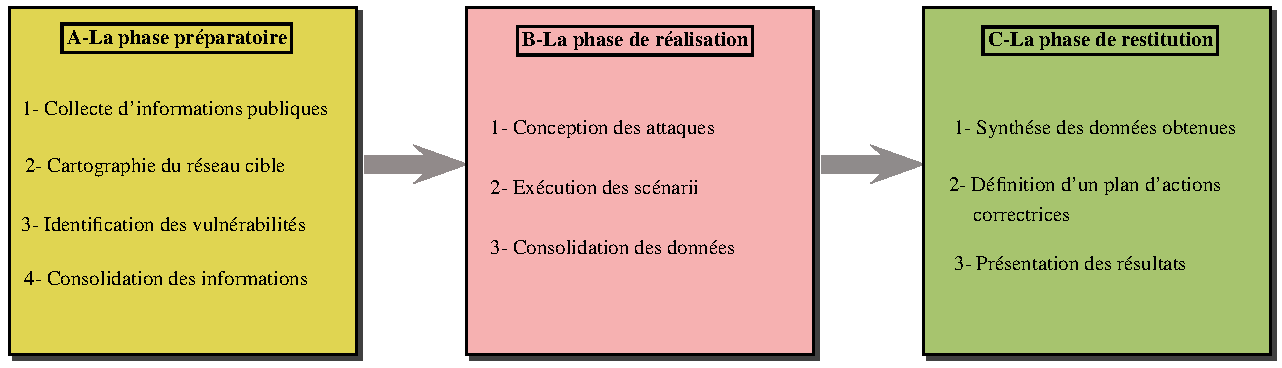
\includegraphics[scale=0.9]{diag1.png}
\caption{\label{intru1}La d�marche utilis�e dans les tests d'intrusion.}
\end{figure}

Nous nous int�ressons ici � la description de la d�marche employ�e
dans les tests d\textquoteright{}intrusion :


\subsubsection*{A. La phase pr�paratoire}
\begin{enumerate}
\item collection d\textquoteright{}informations publiques (DNS, WhoIs, \ldots{})
\item cartographie r�seau de la cible ( ping, traceroute, nmap )
\item identification de vuln�rabilit� (Nessus)
\item consolidation de donn�es obtenues
\end{enumerate}

\subsubsection*{B. La phase de r�alisation}
\begin{enumerate}
\item conception des sc�narii d\textquoteright{}attaques � �valuer
\item ex�cution des sc�narii
\item consolidation des donn�es obtenues
\end{enumerate}
Dans le cas des \textbf{hackers}, l\textquoteright{}intrusion s\textquoteright{}arr�te
ici. Ils nettoient g�n�ralement les traces laiss�es par leur passage.
\\

Dans le cas d\textquoteright{}un audit de s�curit�, il faut alors
fermer les br�ches ouvertes, puis passer � l\textquoteright{}�tape
suivante.


\subsubsection*{C. La phase de restitution}
\begin{enumerate}
\item synth�se des donn�es obtenues lors des phases pr�paratoires puis de
r�alisation
\item d�finition d\textquoteright{}un plan d\textquoteright{}actions correctrices
\item pr�sentation des r�sultats au commanditaire du test
\end{enumerate}
Nous illustrerons dans la suite cette d�marche en indiquant les diff�rents
outils utilis�s agr�ment�s d\textquoteright{}exemples.


\section{L\textquoteright{}audit de vuln�rabilit�}

Nous parlons ici de l\textquoteright{}audit\cite{5} en tant qu\textquoteright{}�tape
de la phase pr�paratoire de la d�marche utilis�e dans les tests d\textquoteright{}intrusion.
Dans le but d\textquoteright{}identifier les failles de vuln�rabilit�, elle consiste � r�cup�rer des informations relatives aux r�seaux et aux syst�mes pr�sents sur ces derniers. Les failles de vuln�rabilit� r�sultent
en g�n�ral de limites jointes � la conception des technologies
ou d�coulent de mauvaises configurations ou utilisations. Les tests
d\textquoteright{}intrusions donnent des indications sur la facilit�
ou � l\textquoteright{}inverse la difficult� d\textquoteright{}acc�der
� l\textquoteright{}information et au syst�me d\textquoteright{}informations
en exploitant les vuln�rabilit�s de s�curit�. Les scanners de vuln�rabilit�
correspondent � une fa�on automatis�e de mise en �vidence de ces failles.
Ils indiquent la fa�on dont il est possible d\textquoteright{}exploiter
ces vuln�rabilit�s et les m�thodes permettant de r�soudre les probl�mes.
Ils couvrent, en g�n�ral, un large �ventail de vuln�rabilit�s connues.
Tandis que les tests d\textquoteright{}intrusion ciblent certaines
vuln�rabilit�s.


\section{Outils li�s aux tests d\textquoteright{}intrusion}

Nous allons reprendre dans cette partie les diff�rentes �tapes de
la d�marche utilis�e dans les tests d\textquoteright{}intrusion que
nous avons pr�sent�es pr�c�demment, dans lesquelles sont utilis�s
des outils sp�cifiques. Nous donnerons �galement des exemples afin
de mieux illustrer la d�marche.

\begin{figure}[!ht]
  \centering
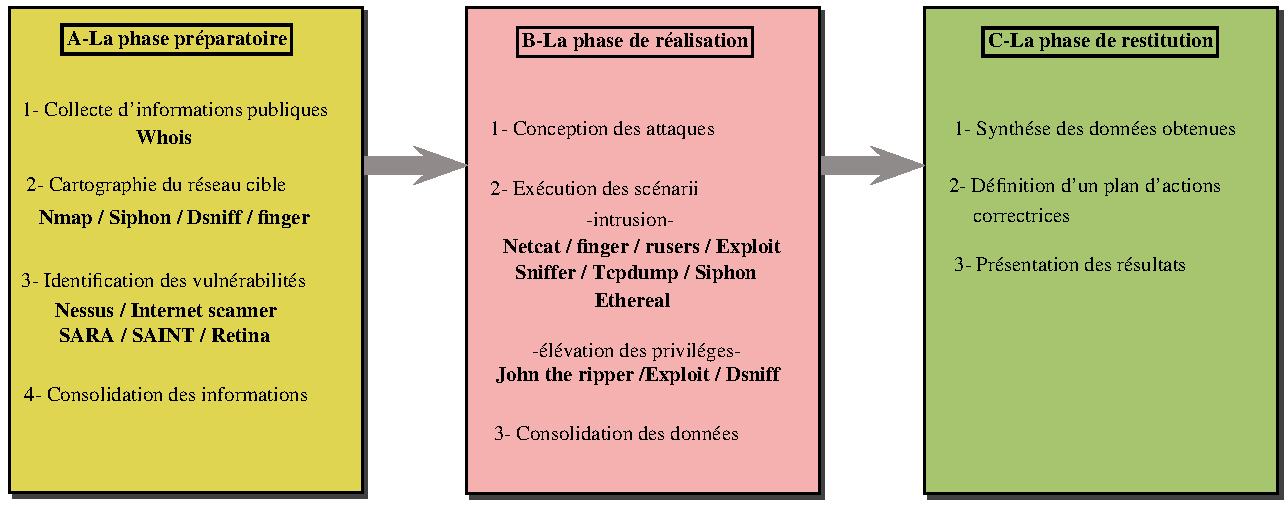
\includegraphics[scale=0.9]{diag2.png}
\caption{\label{intru2}Exemples d'outils utilis�s lors d'une intrusion.}
\end{figure}


\subsection{Divers outils}


\subsubsection{Etape de collecte d\textquoteright{}informations publiques (A.1.)}

La commande \textbf{Whois} permet d\textquoteright{}obtenir des informations
publiques correspondant au r�seau cible : nom du serveur \textbf{DNS},
nom du responsable, num�ro de t�l�phone, adresse e-mail, description
du r�seau etc.


\subsubsection{Etape de cartographie du r�seau cible (A.2.)}

Les outils utilis�s dans cette �tape permettent de r�colter des informations
relatives � la topologie du r�seau afin de d�terminer sa structuration.
Parmi ces outils, nous pouvons trouver :
\begin{description}
\item [{\textbf{\textsl{Nmap}}}] qui est un scanner de r�seau. Il permet
de savoir quels sont les ports ouverts, ferm�s ou filtr�s , ainsi
que le syst�me d\textquoteright{}exploitation autoris� et sa version.
Il permet par exemple de scanner un ensemble d\textquoteright{}\textbf{adresses
IP} en pr�cisant la m�thode de scan utilis�e, les types de ports tels
que les ports \textbf{UDP}, en tentant d\textquoteright{}identifier
la machine cible et en sauvegardant le r�sultat dans un fichier.
\item [{\textbf{\textsl{Siphon}}}] permet de d�couvrir la topologie de
la portion de r�seau sur laquelle se trouve la machine o� nous le
lan�ons. Il indique les syst�mes d\textquoteright{}exploitation pr�sents
sur les machines, les ports ouverts, les machines qui ont le droit
de se connecter au r�seau. Il est ainsi possible de savoir pour quelle
machine nous devons nous faire passer, afin de contourner les Firewalls.
\item [{\textbf{\textsl{Dsniff}}}] permet de visualiser les paquets pr�sents
sur le r�seau et ainsi de r�cup�rer des clefs en sniffant (\textbf{sniffer}).
\item [{\textbf{\textsl{Finger}}}] permet d\textquoteright{}obtenir des
comptes valides. En g�n�ral, le \textbf{d�mon} correspondant est d�sactiv�.
\end{description}


\subsubsection{Etape d\textquoteright{}identification des vuln�rabilit�s (A.3.)}

Nous voulons identifier les failles
potentielles pr�sentes sur le r�seau en utilisant des scanners de
vuln�rabilit� tels que \textbf{Nessus}. L\textquoteright{}utilisation
de ces logiciels n\textquoteright{}est pas tr�s discr�te. En effet,
�tant donn� que ces logiciels testent des failles bien connues des
\textbf{NIDS}, ils sont facilement rep�rables. Les \textbf{NIDS} sont
des syst�mes de d�tection d'intrusion bas�s au niveau d\textquoteright{}un
r�seau. 

Une fois un certain nombre de vuln�rabilit�s est identifi�es, il est alors
n�cessaire d\textquoteright{}�liminer les failles non fond�es. 


\subsubsection{Etape d\textquoteright{}ex�cution des sc�narii (B.2.)}

Dans cette �tape,nous pouvons distinguer deux ensembles de produits utilis�s  ceux qui permettent de s\textquoteright{}introduire sur un
ordinateur ou un serveur et ceux qui permettent de se procurer des
privil�ges auxquels nous n\textquoteright{}avons normalement pas acc�s.



\subsection{Outils d\textquoteright{}audit}

Il ya de nombreux logiciels qui permettent d\textquoteright{}automatiser
la d�couverte de vuln�rabilit�s, ils sont appel�s des scanners. Ils
permettent d\textquoteright{}�valuer les vuln�rabilit�s pr�sentes
sur les r�seaux. Ils se d�clinent sous plusieurs formes et donnent
des r�sultats avec des pr�cisions variables.
\\

Parmi ces logiciels, nous pouvons citer:
\subsubsection{Internet Scanner}

  Il peut s\textquoteright{}int�grer au
produit \textbf{ISS} D�cisions pour �tre utilis� avec d\textquoteright{}autres
produits de s�curit� tels que les syst�mes de d�tection d\textquoteright{}intrusions
et les \textbf{firewall} (pare-feu).


\subsubsection{SATAN, SAINT, SARA}

 SATAN avait la particularit� d\textquoteright{}�tre
\textbf{open source}. Il n\textquoteright{}est plus mis � jour depuis
plusieurs ann�es. Mais, il existe une myriade d\textquoteright{}outils
similaires tel que l\textquoteright{}outil \textbf{open source SARA
}qui est la troisi�me g�n�ration d\textquoteright{}outil d\textquoteright{}analyse
bas� sur \textbf{SATAN}, ou la solution commerciale \textbf{SAINT}.


\subsubsection{Retina}

Nous pouvons �galement citer le logiciel \textbf{Retina}, qui est rapidement devenu populaire. Il analyse le trafic sur
chaque port afin de d�terminer le service utilis�. Il existe une fonction
nomm�e \textbf{CHAM} permettant de d�couvrir de nouvelles failles
de vuln�rabilit�. Cette m�thode repose sur un moteur d\textquoteright{}intelligence
artificiel. \textbf{Retina} est une solution commerciale.


\subsubsection{Nessus, NeWT}

Enfin, il existe une autre offre dont nous allons parler de fa�on
plus approfondie dans ce document, l\textquoteright{}outil Nessus,
et sa version Windows appel�e \textbf{NeWT}. \textbf{Nessus} est un
outil \textbf{open source}. Un fran�ais, renaud Deraison, est l\textquoteright{}auteur
et l\textquoteright{}animateur de se projet. La version Windows est
disponible sur le site de la soci�t� Tenable Network Security en version
d\textquoteright{}�valuation. Nessus semble �tre l\textquoteright{}un
des outils les plus populaires du moment.



\section{conclusion}
Les tests d'intrusion avec ses diff�rents types constituent une tentative autoris�e de simuler les activit�s pour approprier des ressources. Pour cette affaire il existait une d�marche bien pr�cise qui s'est achev�e � l'aide des outils d'audit.
\setcounter{chapter}{3}
\chapter{R�alisation}
\graphicspath{{Chapitre4/figures/}}

%==================================================================================================%

\section{Introduction}
Suite � l'�tude �labor�e dans les trois chapitres pr�c�dents on a atteint la derni�re phase de la r�alisation de nos tests. Ce chapitre est destin� pour d�crire cette phase et pr�senter les r�sultats aux quels on a aboutit.
Nous commencerons d'abord par pr�senter les diff�rents outils techniques � utiliser pour r�aliser le travail.



\section{Environnement de travail}


\subsection{Environnement matri�l}

La plate-forme de travail est une machine de caract�ristique suivantes :
\begin{maliste}

\item Processeur : Intel core 2 duo 2.00 GHz
\item RAM : 2043 Mo
\end{maliste}

\subsection{Environnement logiciel}

Syst�me d'exploitation :
\begin{maliste}

\item Windows vista Edition familial premium
\item Windows Xp sp2
\item Mandriva Linux 2009 spring 
\item Linux Backtrack 4 beta
\end{maliste}
Machine virtuelle :
\begin{maliste}

\item VMware Workstation v6.0.3
\item Sun VirtualBox v3.1.6
\end{maliste}
Et LATEX comme environnement de r�daction du rapport.


\subsection{Back|Track}


\subsubsection{L\textquoteright{}outil}

BackTrack \cite{6} est une distribution GNU/Linux bas�e sur la distribution
\textit{Slackware} jusqu'� la version 3 et \textit{Ubuntu} depuis
la version 4 apparue en 11 Janvier 2010. Son objectif est de fournir
une distribution regroupant l'ensemble des outils n�cessaires aux
tests de s�curit� d'un r�seau.

Avec ces 300 outils, BackTrack aborde tous les domaines li�s aux s�curit�s
modernes allant de l\textquoteright{}audit r�seau � l\textquoteright{}analyse
et l\textquoteright{}identification de vuln�rabilit�s en passant par
divers outils de r�cup�ration d\textquoteright{}informations. (\textbf{Fuzzers}
/ Testeurs de s�curit� des r�seaux filaires / Testeur des r�seaux
\textbf{wifi} ...)

BackTrack est principalement connu et utilis� � des fins d\textquoteright{}audit
de r�seaux sans fil wifi. Son d�veloppement est ax� sur la prise en
charge de cartes wifi supportant le mode Monitoring, ce qui permet
la capture de paquets, n�cessaire pour le crack de cl� \textbf{WEP}/
\textbf{WPA} et autres test (suite de logiciel aircrack-ng par exemple)

BackTrack contient aussi des applications basiques comme un lecteur
multim�dia, traitement de texte ... ce qui en fait un syst�me d\textquoteright{}exploitation
polyvalent.


\subsubsection{Installation}

L\textquoteright{}un des principaux int�r�ts de BackTrack est d'�tre
disponible sous forme d'un Livecd, c'est � dire qu\textquoteright{}un
ordinateur peut booter directement sur le cd sans avoir � se pr�occuper
d\textquoteright{}une quelconque installation avec la possibilit�
d\textquoteright{}ex�cuter chaque outil imm�diatement.

Ainsi, tout se passe dans la m�moire RAM de l\textquoteright{}ordinateur
n\textquoteright{}entrainant aucune intervention sur le disque dur
permettant ainsi de l\textquoteright{}utiliser sans risque de perte
de donn�es ou autre. Ce Livecd permet d\textquoteright{}avoir tous
les outils indispensables � la s�curit� informatique sans laisser
aucune trace.


\subsubsection{Tests qu'on peut r�aliser}

Comme nous avons pu le dire pr�c�demment, l\textquoteright{}objectif
de BackTrack est de fournir une distribution compacte regroupant le
maximum d\textquoteright{}outils n�cessaire aux tests de s�curit�
d\textquoteright{}un r�seau ou d\textquoteright{}application.

Le nombre d\textquoteright{}outils li�s � la s�curit� informatique
ne cesse de cro�tre avec les versions de BackTrack.
\\

Dans la version 4.0 beta, nous disposons d\textquoteright{}approximativement
300 outils d�compos�s en 16 cat�gories. Voici les parties qu\textquoteright{}il
nous est possible d\textquoteright{}utiliser dans de nombreux cas
:


\subsubsection*{Analyse de r�seau sans fil}
\begin{description}
\item [{\textit{Aircrack-ng,wesside-ng}}] pour l\textquoteright{}analyse
et le crackage de Wifi.
\item [{\textit{BTscanner,BlueSnarfer}}] pour l\textquoteright{}analyse
et le crackage de Bluetooth.
\end{description}

\subsubsection*{Anonymat}
\begin{description}
\item [{\textit{TOR}}] permet d\textquoteright{}�tre compl�tement invisible
sur le net sans laisser la moindre trace � fin d\textquoteright{}�viter
de nombreux d�m�l�s judiciaires, il peut �tre une bonne chose de ne
pas laisser de traces sur les diff�rents syst�mes comme dans les fichiers
de \textbf{logs} par exemple.
\end{description}

\subsubsection*{Attaque de mot de passe}

BackTrack dispose d\textquoteright{}un large panel de possibilit�
d\textquoteright{}attaque contre les mots de passe que ce soit des
attaques << en ligne >> ou bien << locale >>.
\begin{description}
\item [{\textit{Hydra}}] concernant les attaques en lignes , il est actuellement
consid�r� comme l\textquoteright{}un des meilleurs brute forceur en
ligne.
\item [{\textit{RaimbowCrack}}] Concernant les attaques hors lignes, il
est un casseur de mot de passe bas� sur les raimbows tables ce qui
le rend excessivement puissant.
\end{description}

\subsubsection*{Collecte d\textquoteright{}informations}

Il faut toujours prendre tr�s au s�rieux cette partie qui est la base
de toute attaques de petite ou de grande envergure. Suivant le type
d\textquoteright{}informations que nous d�sirons rechercher, nous
avons la possibilit� de choisir parmi les nombreux outils que nous
propose BackTrack.
\begin{description}
\item [{\textit{Wapiti}}] nous permettre de r�cup�rer des informations
sur les failles Web
\item [{\textit{Nessus}}] nous permettre de visualiser les vuln�rabilit�s
d\textquoteright{}un syst�me d\textquoteright{}exploitation ainsi
que ces services
\item [{\textit{Nmap}}] simplement nous renseigner sur les ports ouverts
\end{description}

\subsubsection*{P�n�tration}

l\textquoteright{}�tape suivant la r�cup�ration d\textquoteright{}information
est en r�gle g�n�rale la p�n�tration de la cible. 
\begin{description}
\item [{\textit{M�tasploit}}] Il contient une base de donn�es d\textquoteright{}environ
300 exploits, capable de simplifier les tests d'intrusion sur des
failles importantes.
\end{description}

\subsubsection*{Reverse engineering}

C'est l'activit� qui consiste � �tudier un programme pour en d�terminer
le fonctionnement interne ou sa m�thode de fabrication afin de pouvoir
par exemple s\textquoteright{}octroyer des acc�s ou des fonctionnalit�s
ne nous �tant pas autoris� initialement.
\begin{description}
\item [{Ollydbg}] outils tr�s performant en mati�re de cracking pour d�bogueur/d�sassembleur
\item [{Hexedit}] comme �diteur hexad�cimal
\end{description}

\subsubsection*{Sniffers}

les sniffers sont des logiciels qui peuvent r�cup�rer les donn�es
transitant par le biais d'un r�seau local.
\begin{maliste}

\item Dsniff 
\item Ettercap-ng(anciennement Ettercap)
\item Wireshark(anciennement Ethereal)
\end{maliste}

\subsubsection{Evolutions}

BackTrack est � l\textquoteright{}heure actuelle la distribution la
plus aboutie en mati�re de s�curit� informatique. BackTrack se qualifient
tant par le nombre impressionnant d\textquoteright{}outils que leur
par qualit� reconnu par les professionnels. Ces nombreux d�veloppeurs
et sa large communaut� permettent d\textquoteright{}avoir une distribution
de plus en plus stable avec une compatibilit� accrue avec les diff�rents
constructeurs de mat�riels. BackTrack a gagn� une grande notori�t�
et c\textquoteright{}est pourquoi, en 2006, BackTrack a �t� �lu comme
�tant la premi�re distribution de s�curit� par \href{http://insecure.org}{insecure.org}.


\section{Les tests r�alis�s}

Apr�s la d�finition de diff�rents outils technique et environnements
de tests pour l'ach�vement de ce travail nous allons dans ce qui suit
pr�senter les taches et les tests r�alis�s. 

Nous allons dans cette partie effectuer une s�rie de tests � l\textquoteright{}aide
de Backtrack. Suite � des contraintes de type mat�riel, la strat�gie
adopt�e est une strat�gie de type interne. Le client et le serveur
sont tous deux situ�s � l\textquoteright{}int�rieur d\textquoteright{}un
r�seau local \textbf{Ethernet}. L\textquoteright{}objectif est de
mieux appr�hender ce qui sont les failles de s�curit� dans un tel
r�seau au travers de tests simples.

\subsection{Topologie}

\begin{figure}[!ht]
  \centering
\includegraphics[scale=1.0]{Rvirtuelle.png}
\caption{\label{chap4-1}Le r�seau Ethernet utilis� pour les tests}
\end{figure}

Nous avons cr�� 3 machines virtuelles sur VMware, pour qu\textquoteright{}elles
puissent communiquer directement sur le r�seau physique. Pour ce l�,
nous avons utilis�s le mode \textbf{Host-Only} qui permet de connecter
les cartes r�seau (virtuelles) des VM directement � la carte physique.
Cette connexion permet entre autres d\textquoteright{}activer le service
\textbf{DHCP-Server}, afin de d�livrer des adresses \textbf{IP} aux
machines virtuelle du r�seau \textbf{Host-Only}. Du point de vue de
la \textbf{VM}, c\textquoteright{}est comme si elle �t� directement
connect�e au r�seau physique. Techniquement, un \textbf{vHUB} est
cr�e, et est connect� � la carte r�seau physique, via l\textquoteright{}interface
associ�e. Ceci explique pourquoi il est possible d\textquoteright{}utiliser
des sniffeurs de paquets directement sur l\textquoteright{}interface
dans le but d\textquoteright{}�couter le trafic r�seau des machines
virtuelles.


Diff�rents syst�mes ont �t� install�s sur ces machines virtuelles.
Les configurations de ces derniers ont �t� indiqu�es dans le tableau tab\ref{tabutil}


\begin{table}[!ht]

\begin{center}
\begin{tabular}{|c|c|c|c|c|}
\hline 
\multicolumn{2}{|c|}{\textbf{\small V.M.}} & \textbf{\small VM-1} & \textbf{\small VM-2} & \textbf{\small VM-3}\tabularnewline
\hline
\multicolumn{2}{|c|}{\textbf{\small Adresse IP}} & 192.168.56.102 & 192.168.56.104 & 192.168.56.101\tabularnewline
\hline 
 & {\small Type de carte} & {\small PCnet-FAST III } & {\small PCnet-FAST III } & {\small PCnet-FAST III }\tabularnewline
\textbf{\small Carte r�seau} &  & {\small (Am79C793)} & {\small (Am79C793)} & {\small (Am79C793)}\tabularnewline
\cline{2-5} 
 & {\small Adresse MAC} & {\small 08 00 27 1F 04 70} & {\small 08 00 27 1C 73 44} & {\small 08 00 27 2B 50 FD}\tabularnewline
\hline 
\multicolumn{2}{|c|}{\textbf{\small M�moire vive}} & {\small 512 Mo} & {\small 256 Mo} & {\small 256 Mo}\tabularnewline
\hline 
\multicolumn{2}{|c|}{\textbf{\small OS}} & {\small Linux Backtrack 4 beta} & {\small Linux Mandriva } & {\small Windows XP-sp2}\tabularnewline
\hline
\end{tabular}
\caption{Les configurations des machines virtuelles }
\label{tabutil}
\end{center}
\end{table}

\textbf{\textit{NB}} : cette topologie n'est valable que pour les
deux premiers test (test 1 et test 2 ).


\subsection{Les tests r�alis�s}


\subsubsection{Test 1 : Scan de vun�rabilit� }

Le but de ce scan est de d�tecter des failles de s�curit� potentielles
dans les machines d'un r�seau. En effet l' identification des vuln�rabilit�s
est inclue dans la phase pr�paratoire de la d�marche utilis�e dans
les tests d\textquoteright{}intrusion. Il y a diff�rents scanners
de vuln�rabilit� (payants et non payants), dont un seul sera examin�.
\\

Alors, on a choisi Nessus, qui est un programme non payant fonctionnant
avec un mod�le client-serveur, pour effectuer ce test. Il nous fournira
des rapports d�taill�s et nous informera si notre ordinateur test�
comporte des failles de s�curit� (Nessus v4.2 dispose d\textquoteright{}une
base de 35973 plugins couvrant ainsi un nombre de failles impressionnantes)
et proposera m�me des solutions pour ces failles.


\subsubsection*{Param�trage}
Ce premier essai est r�alis� sur une machine Linux VM-3, ayant comme
services un serveur de types SSH, FTP,SMTP, HTTP et HTTPS. Les param�tres
du test sont comme suit : 
\begin{maliste}
\item Nessus 4.2 (version Windows) est install� sur la machine VM-3 en 2
�tapes : 

\begin{maliste}
\item installation le logiciel et ses plugins
\item cr�ation d'un nouveau compte utilisateur dans Nessus Server Manager
\end{maliste}
\item Les essais vont �tre effectu�s depuis le client Nessus (d�j� install�
avec le serveur) se trouvant dans VM-3 et plus pr�cis�ment dans l'adesse <<
https://127.0.0.1:8834/ >>. 
\item La machine cible est VM-2.
\end{maliste}
pour lancer le scan il faut suivre les 2 �tapes :


\subsubsection*{\textit{�tapes 1 : Ajouter une politique de scan}}

L'ajout d'une politique de scan avec \textquotedblleft{} Add Policy
\textquotedblright{}(voir fig \ref{chap4plice}) nous permet :



\begin{maliste}
\item d'indiquer le choix des scanners de port utilis�(1). 
\item d'�viter de faire tomber le serveur cibl� par l'activation de l\textquoteright{}option
<< safe checks >>(2).
\item choisir le nombre d\textquoteright{}ordinateurs � tester en m�me temps(3).
\item possibilit� d'activer ou de d�sactiver les plugins de scan
(35980 plugins distribu�s en 42 familles).
\end{maliste}

\begin{figure}[!ht]
  \centering
\includegraphics[scale=0.50]{policiermod.png}
\caption{\label{chap4plice}La fen�tre d'ajout de polilitic de scan \textquotedblleft{}Edit Policy\textquotedblright{}}
\end{figure}


\subsubsection*{\textit{�tapes 2: Ajouter un scan}}

L'ajout du scan avec \textquotedblleft{} Add Scan \textquotedblright{}(voir fig \ref{scann}) se r�alise par :
\begin{maliste}
\item donner un nom du scan \textquotedblleft{}scan du machine VM-1\textquotedblright{}(1)
\item choisir la politique du scan(2)
\item donner l'adresse IP du machine VM-3 \textquotedblleft{}192.168.56.104\textquotedblright{}(3)
\end{maliste}

\begin{figure}[!ht]
  \centering
\includegraphics[scale=0.66]{scann.png}
\caption{\label{scann}La fen�tre d'ajout de scan \textquotedblleft{}Edit Scan\textquotedblright{}}
\end{figure}

\subsubsection*{Exploitation}

Lors du lancement, le programme va scanner tous les ports de la machine
pour conna�tre les services qui sont disponibles, puis les essais
de vuln�rabilit� commencent : le test a dur� environ 5 minutes. Le
r�sultat de scan est visible sur la Figure \ref{scan6mod}, mais on peut constater
que ce n\textquoteright{}est pas tr�s parlant. Alors il est possible
de sauver ce test en s�lectionnant le bouton {}`` Download '' (1)et
en indiquant le type de format : HTML, .nessus , .nessus (v1).
\\

Il est pr�f�rable de sauver sous le format HTML, de cette mani�re
il est possible d\textquoteright{}analyser les vuln�rabilit�s du syst�me
facilement. Sur cette page HTML sont expliqu�s le type d\textquoteright{}attaque
des vuln�rabilit�s et les solutions. 
\\
Voici ce qui est dit au sujet du serveur FTP : il �tait possible de
mettre hors service le serveur FTP en faisant 3000 connections sur
celui-ci : un attaquant peut employer ce d�faut pour emp�cher ce service
de travailler correctement. Et la solution � ce probl�me est de t�l�charger
la mise � jour du serveur.Ainsi, une telle explication est faite �
chaque vuln�rabilit� d�tect�e.

\begin{figure}[!ht]
  \centering
\includegraphics[scale=0.50]{scan6mod.png}
\caption{\label{scan6mod}R�sultat d'analyse du machine VM-2 }
\end{figure}


\subsubsection{Test 2 : Sniffer le traffic r�seau}

� fin de r�cup�rer les mots de passe circulant dans le flux de notre
r�seau ou\textquoteright{} la grande majorit� des protocoles font
transiter les informations en clair, c\textquoteright{}est-�-dire
de mani�re non chiffr�e. Ainsi, lorsqu\textquoteright{}un utilisateur
du r�seau consulte un serveur via le protocole \textbf{FTP} ou \textbf{SFTP}, ou acc�der
sur des sites dont l\textquoteright{}adresse commence par \textbf{HTTP} ou
\textbf{HTTPS}, toutes les informations envoy�es ou re�ues peuvent �tre intercept�es.
\\

On va utilis�e :
\begin{maliste}

\item \underbar{Wireshark} pour r�cup�rer les mot de passe circulant dans
les paquets \textbf{FTP} et \textbf{HTTP}
\item \underbar{Ettercap} pour r�cup�rer les mot de passe circulant dans
les paquets \textbf{FTPS} et \textbf{HTTPS}
\end{maliste}
Suite au r�sultat obtenue par le Test 1, on a constat� que le port
\textbf{FTP} est ouvert ce qui nous a donn� la possibilit� de r�cup�rer un
login et son mot de passe pour acc�der au serveur \textbf{FTP}.


\subsubsection*{\underbar{ 2-A : En utilisant Wireshark}}


\subsubsection*{Param�trage}
\begin{maliste}

\item le sniffeur est installer dans VM-1 � fin de capturer le traffic entre VM-2
et VM-3.
\item le serveur \textbf{FTP} (ou Web) est installer dans le VM-2.
\item le client \textbf{FTP} (ou Web) est le VM-3.
\end{maliste}

\subsubsection*{Exploitation}
\begin{enumerate}
\item On lance la capture des trame dans l'analyseur Wireshark dans VM-1.
\item On fait un test de connection, par login et mot de passe, du client
VM-3 au serveur VM-2(l'adresse est ftp://192.168.56.104/).
\item On fait le filtrage des paquets en capture et impression (avec personnalisation
de l\textquoteright{}utilisation de la couleur) 
\end{enumerate}
voici le d�tail des �changes entre le client et le serveur :

\begin{figure}[!ht]
  \centering
\includegraphics[scale=0.66]{capture1.jpg}
\caption{\label{chap4-2}Capture du traffic entre le client FTP et le serveur FTP avec Wireshark}
\end{figure}

On peut s'apercevoir que dans les �changes, les ligne avec l'ID entre
28 et 33 contient l'identifiant et le mot de passe de l'utilisateur
\textbf{FTP} situ� dans VM-1. 


\subsubsection*{\underbar{Test 2-B : En utilisant Ettercap}}


\subsubsection*{Param�trage}
\begin{maliste}

\item le sniffeur est installer dans VM-1

\begin{itemize}
\item sa configuratuion par la commande : {}``vim /etc/etter.conf''
\end{itemize}
\item le serveur Web s�curis� (ou FTP s�curis�e) est installer dans le VM-2.
\item le client Web s�curis� (ou FTP s�curis�e) est le VM-3.
\end{maliste}

\subsubsection*{Exploitation}
\begin{enumerate}
\item On lance le sniffeur par la commande :
\begin{verbatim}
ettercap -TqM ARP :REMOTE /192.168.56.101/ / 192.168.56.104/
\end{verbatim}
 
\item On fait le m�me test de connection dans le Test 2-A (l'adresse est
ftp://192.168.56.104/).
\item De plus on fait aussi un test de connection sur le serveur web s�curis�(l'adresse
est https://192.168.56.104/toto/secr.php). 
\end{enumerate}

Comme r�sultat, Ettercap nous donne les logins(USER ) et leurs
mot de passe(PASS). Il distingue automatiquement les mots de passe
et les logins. Les r�sultats des �changes entre le client et
le serveur dans la figure \ref{chap4-3}.

\begin{figure}[!ht]
  \centering
\includegraphics[scale=0.8]{ettercap.png}
\caption{\label{chap4-3}Capture du traffic entre le client FTP et le serveur FTP avec Ettercap}
\end{figure}



\subsubsection{Test 3 : Crackage d\textquoteright{}un cl� WEP dans un r�seau sans
fil (Wi-Fi)}

La technologie sans fil\cite{Cederic} Wi-Fi (IEEE 802.11) s\textquoteright{}appuie
sur les ondes hertziennes pour �tablir les communications entre les
�quipements. Il suffit de se trouver dans la zone de couverture des
�metteurs pour �couter les donn�es.Ainsi, Le protocole \textbf{WEP}
chiffre chaque trame 802.11 �chang�e entre l\textquoteright{}�metteur
et le r�cepteur (point d\textquoteright{}acc�s ou client).
\\

Il existe plusieurs m�thodes pour casser une cl� WEP. On cite le processus
de crackage par Aircrack-ng. La suite aircrack-ng comprend plusieurs
programmes dont les 3 principaux sont : 
\begin{lyxlist}{00.00.0000}
\item [{\textbf{Airodump-ng}}] le logiciel de capture de paquets, c'est lui qui
scan les r�seaux et conserve les paquets qui serviront � d�crypter
la cl�.
\item [{\textbf{Aireplay-ng}}] un logiciel dont la principale fonction est l'envois
de paquets dans le but de stimuler le r�seau et capturer plus de paquets.
\item [{\textbf{Aircrack-ng}}] le logiciel de crack de cl�, c'est un logiciel qui
� partir des informations captur�es � l'aide d'airodump va nous donner
la cl� (si on en a eu un nombre suffisant de paquets).
\end{lyxlist}
le processus d'attaque est situ� dans la figure \ref{chap4-4}

\begin{figure}[!ht]
  \centering
\includegraphics[scale=1]{lesphase.jpg}
\caption{\label{chap4-4}le processus de crackage du cl� Wi-Fi}
\end{figure}


\subsubsection*{Param�trage}
\begin{maliste}

\item M-1 est la machine du test de crackage qui a les m�me param�tre que
VM-1 avec une carte wifi \textit{chipset atheros} .
\item Le point d'acc�s est R, un routeur wifi connect� � l'Internet .
\item Une machine M-2 d�ja connect� avec le point d'acc�s R par la cl� secr�te,
alors il y'a des �changes de paquets entre ces derniers.(voir fig \ref{chap4-5}
)
\end{maliste}

\begin{figure}[!ht]
  \centering
\includegraphics[scale=0.66]{terminaux.png}
\caption{\label{chap4-5}Le r�seau du test 3 }
\end{figure}

\subsubsection*{Exploitation }


\subsubsection*{\textit{Phase 1}}

On commence � chercher le r�seaux wifi voulu avec airodump par la
commande : 
\begin{verbatim}
airodump-ng interface
\end{verbatim}

Une fois lanc� airodump,
on se trouve dans l'interface indiqu� dans la figure

%%%%%%%%%%%%%%%%%%%%%%%%%%%%%%%%%%%%%%%%%%%%%%

\begin{figure}[!ht]
  \centering
\includegraphics[scale=0.66]{air1.png}
\caption{\label{chap4-7}le processus de crackage du cl� Wi-Fi}
\end{figure}

\begin{maliste}

\item La colonne \textbf{BSSID} correspond � l'adresse mac des points d'acc�s
(R)
\item La colonne \textbf{ESSID} correspond au nom du r�seau
\item La colonne \textbf{power} donne une indication de la puissance de
reception, cette information peut foirer (-1) cela n'influ en rien
la puissance de reception r�elle , une bonne indication est la vitesse
de d�filement des beacons
\item La  partie (1) correspond aux points d'acc�s et la seconde partie
aux stations ( l' ordinateur qui se connecte � R c'est M-2).
\item Airodump nous indique dans la colonne \textbf{ENC} le cryptage utilis�
(WEP, WPA, OPN).On choisie notre r�seau crypter par WEP.
\item La colonne qui nous int�resse est la colonne des \textbf{IVs}, la
colonne \textbf{\#data}, c'est ces \textquotedbl{}bouts de fichiers\textquotedbl{}
qui vont nous permettre de cracker notre cl� wep aucun rapport avec
la colonne beacons completement inutile pour le crack.
\end{maliste}

\subsubsection*{\textit{Phase 2 et 3 :} }

Lancer le scann apr�s avoir choisie le r�seau par la commande : 
\begin{verbatim}
airodump-ng --write NomFichierSortie --channel NumeroChannel -b @mac_R Interface
\end{verbatim}
Dans notre cas:
\begin{verbatim}
airodump-ng --write tuto --channel 11 -b 02:1F:3B:00:09:2D ath0
\end{verbatim}
dont les param�tres sont:
\begin{maliste}
\item \textquotedbl{}\textit{--write tuto}\textquotedbl{} \textit{--write} indique que l'on
souhaite enregistrer la capture, il est suivis du nom du fichier dans
lequel on l'enregistre justement.
\item \textquotedbl{}\textit{--channell XX}\textquotedbl{} Indique sur quel channel
on scan.
\end{maliste}
Il est necessaire de connaitre l'adresse mac d'un ordinateur (station)
d�ja accept� par le point d'acc�s R (dans notre cas l'odinateur est
M-2) car Pour aireplay, le programme qui va envoyer des paquets, a
justement besoin de l'adresse mac de M-2. En fait, on se fait passer
pour l'ordinateur M-2 qui a le droit d'acc�s au point d'acc�s R en
spoofant son adresse mac pour pouvoir par exemple injecter des paquets
ensuite.


\subsubsection*{\textit{Phase 4}}

Maintenant que l'on sait que le cryptage est WEP, qu'une station est
pr�sente et qu'il y a du trafic (quelques data en peu de temps), on
va lancer aireplay, un injecteur de paquets pour acc�l�rer le trafic
et surtout stimuler les IVs.
\begin{maliste}
\item On va en premier lieu tester l'association avec le point d'acc�s avec
une attaque \textquotedbl{}-1\textquotedbl{} dite de fake authentication.Cette
�tape n'est pas indispensable, elle peut servir � tester si le point
d'acc�s poss�de un filtrage d'addresse mac. La synthaxe est la suivante:

\begin{verbatim}
aireplay-ng -1 0 -e ESSID -a @mac_R -h @mac_M-2 interface
\end{verbatim}

\begin{maliste}

\item << \textit{-1 0} >> -1 indique une fake authentication
et 0 indique le temps a laisser entre 2 tentatives (ici nul).
\item << \textit{-e ESSID} >> ici il faut remplacer ESSID
par le nom du reseau colonne ESSID.
\item << \textit{-a adresse-mac-de-R} >> colonne BSSID.
\item << \textit{-h adresse-mac-de-M2} >> colonne
STATION.
\item << \textit{interface} >> a remplacer par le nom de
votre interface (rausb0, ath1 ...)
\end{maliste}
\item En deuxi�me lieu, on va faire des injections de paquets. Elle est la
cl� pour r�ussir cette crack wep rapidemment. En effet il est necessaire
de capturer beaucoup de Ivs pour trouver la cl� wep. L'attaque la
plus prolifique pour g�n�rer des Ivs est l'attaque << -3 >>
dite de r�injection d'ARP : 
\begin{verbatim}
aireplay-ng -3 -e ESSID -b @mac_R -h @mac_M-2 interface
 \end{verbatim}
\end{maliste}
Aireplay nous sauvegarde donc les arp captur�s dans un fichier qu'il
cr�� � chaque fois qu'il est lanc�. Ce fichier se trouve dans le r�pertoire
� partir duquel nous avons lanc� airplay.


\subsubsection*{\textit{Phase 5}}

Sachant qu'il faut environ 300 000 IVs pour cracker une cl� wep 64bits
et environ de 1 000 000 pour une cl� wep 128, cette phase est la
plus importante de tout le processus du crackage.
\\

On lancant aircrack-ng par 
\begin{verbatim}
aircrack-ng -x *.cap *.ivs 
 \end{verbatim}

\begin{figure}[!ht]
  \centering
\includegraphics[scale=1]{air2.png}
\caption{\label{chap4-6}R�sultat obtenu par Aircrack-ng }
\end{figure}

Il nous affiche tous les r�seaux qu'il a rencontr�, leur cryptage
et le nombre de IVs correspondant (voir chap4-6). Il suffit
d'entrer le num�ro de notre r�seau, de lancer aircrack et il commence
� cracker la cl� wep. Apr�s une attente, on a obtenue le mot de
passe d�crypt� << Decrypted correctly : 100\% >>


\subsubsection*{\textit{Phase 6}}
Cette phase n'est qu'un test du cl� crypt�e si elle est la bonne ou non. Alors ce n'est qu'une demande � rejoindre 
le r�seau et d'utiliser les ressources disponibles: Acc�s Internet, Partage de fichier... 

\section{Conclusion}
  
Dans ce chapitre, nous avons pu mettre en �vidence quelques exemples d'utilisation des outils d'analyse r�seaux, de test de vuln�rabilit� et des tests d'intrusion. Ces outils ont une diversit� d'utilisation et une multitude de fonctionnalit�s que nous n'avons pas pu les explorer tous.

\backmatter
\pagestyle{fancy}
\fancyhf{}
\renewcommand{\chaptermark}[1]{\markboth{Conclusion g�n�rale et perspectives}{}}
\fancyhead[R]{Conclusion g�n�rale et perspectives}
\fancyfoot[R]{\thepage}
%\fancyfoot[LE]{\thepage}
\renewcommand{\headrulewidth}{0.5pt}
\renewcommand{\footrulewidth}{0pt}
\chapter{Conclusion g\'en\'erale et perspectives}


Dans le cadre de ce projet qui nous a �t� tr�s b�n�fique, a enrichit
nos connaissances et apr�s une premi�re exp�rience dans un domaine
vaste et complexe de la s�curit� des r�seaux, nous sommes arriv�s
� effectuer une analyse d'un r�seau avec une etude des differents
outils d'analyse du r�seau, un scan de vuln�rabilit� moyenant l'outil
Nessus et un test d'intrusion.
\\

Ce sujet a �t� motivant et passionnant. Il nous a permis d'approfondir
nos connaissances pour tout se qui conserne la s�curit� informatique.
En effet les nouveaux logiciels ne sont pas toujours au point et nous
avons d� beaucoup acc�der aux forums de discussion pour r�soudre des
bugs. Nous avons appris � ne pas nous d�courager et � contourner les
difficult�s et aller jusqu'au bout de soi.
\\

Comme perspective d'�volution, ce projet peut �tre perfectible, en
utilisant d'une mani�re plus pouss� l'outil Backtrack pour faire des
tests d'intrusion sur des syst�mes d'information, des bases de donn�es
et des sites Web. Ceci peut faire l'objectif d'un nouveau PFA.
\appendix
\setcounter{figure}{0} 
\setcounter{table}{0}
\setcounter{footnote}{0}
\setcounter{equation}{0}
\pagestyle{fancy}
\fancyhf{}
\renewcommand{\chaptermark}[1]{\markboth{\MakeUppercase{#1 }}{}}
\renewcommand{\sectionmark}[1]{\markright{\thesection~ #1}}
\fancyhead[R]{\bfseries\leftmark}
%\fancyhead[LE]{}
\fancyfoot[R]{\thepage}
%\fancyfoot[LE]{\thepage}
\renewcommand{\headrulewidth}{0.5pt}
\renewcommand{\footrulewidth}{0pt}

\makeatletter
\renewcommand\thefigure{A.\arabic{figure}}
\renewcommand\thetable{A.\arabic{table}} 
\makeatother

\chapter{Annexe A : Glossaire}
\graphicspath{{Annexe1/figures/}}
%==========================================================================

%    Annexe

%===========================================================================
\begin{lyxlist}{00.00.0000}
\item [{\textbf{ACK}}] Signale que le paquet est un accus� de r�ception
(ACKnowledgement)
\item [{\textbf{ARP}}] Address Resolution Protocol, protocole de r�solution
d'adresse
\item [{\textbf{ASCII}}] Code Americain Standard pour l'Echange d'Informations
\item [{\textbf{ASP}}] Active Server Pages, est un ensemble de logiciels
d�velopp�s par Microsoft et utilis�s dans la programmation Web
\item [{\textbf{Cookie}}] est d�fini par le protocole de communication
HTTP comme �tant une suite d'informations envoy�e par un serveur HTTP
� un client HTTP
\item [{\textbf{d�mon}}] un processus charg� d'une mission (par exemple
g�rer un p�riph�rique ou le r�seau)
\item [{\textbf{DHCP}}] Dynamic Host Configuration Protocol
\item [{\textbf{DHCP-Server}}] Dynamic Host Configuration Protocol Serveur 
\item [{\textbf{DNS}}] Domain Name System (ou DNS, syst�me de noms de domaine) est
un service permettant d'�tablir une correspondance entre une adresse
IP et un nom de domaine
\item [{\textbf{Ethernet}}] est un protocole de r�seau local � commutation
de paquets
\item [{\textbf{FDDI}}] Fiber Distributed Data Interface (FDDI) est un type de r�seau informatique LAN ou MAN permettant d'interconnecter plusieurs LAN � une vitesse de 100 Mbit/s sur de la fibre optique
\item [{\textbf{Firewall}}] pare-feu , prot�geant des intrusions dans un
r�seau
\item [{\textbf{Fuzzers}}] est une technique pour tester des logiciels
par bo�te noire
\item [{\textbf{GUI}}] Interface graphique
\item [{\textbf{hackers}}] utilis� pour d�signer en informatique les programmeurs
astucieux et d�brouillards
\item [{\textbf{Host-Only}}] mode de connexion permet la communication
entre les machines virtuelles et l\textquoteright{}h�te de virtualisation
uniquement, rien ne sort sur le r�seau physique.
\item [{\textbf{HTTP}}] HyperText Transfer Protocol
\item [{\textbf{HTTPS}}] HyperText Transfer Protocol secured
\item [{\textbf{ICMP}}] Internet Control Message Protocol
\item [{\textbf{IDS}}] Intrusion Detection System
\item [{\textbf{IMAP}}] Internet Message Access Protocol
\item [{\textbf{IP}}] Internet Protocol
\item [{\textbf{ISS}}] Internet Security System
\item [{\textbf{IV}}] Initialization Vector 
\item [{\textbf{LAN}}] Local Area Network. R�seaux locaux. R�seau situ� dans une zone r�duite ou dans un
environnement commun, tels qu'un immeuble ou un bloc d'immeubles.
\item [{\textbf{LDAP}}] Lightweight Directory Access Protocol est � l'origine un protocole permettant l'interrogation et la modification des services d'annuaire.
\item [{\textbf{Mode-promiscuous}}] se r�f�re � une configuration de la
carte r�seau, qui permet � celle-ci d'accepter tous les paquets qu'elle
re�oit, m�me si ceux-ci ne lui sont pas adress�s.
\item [{\textbf{NIDS}}] Network Intrusion Detection System
\item [{\textbf{open-source}}] code source libre, s'applique aux logiciels
dont la licence respecte des crit�res pr�cis�ment �tablis par l'Open
Source Initiative
\item [{\textbf{Perl}}] un langage de programmation, reprenant des fonctionnalit�s
du langage C et des langages de scripts sed, awk et shell (sh).
\item [{\textbf{PHP}}] Hypertext Preprocessor,est un langage de scripts
libre principalement utilis� pour produire des pages Web dynamiques
via un serveur HTTP
\item [{\textbf{POP}}] Post Office Protocol, est un protocole qui permet
de r�cup�rer les courriers �lectroniques situ�s sur un serveur de
messagerie �lectronique
\item [{\textbf{R�tro-ing�nierie}}] ing�nierie inverse, est l'activit� qui consiste � �tudier un objet pour en d�terminer le fonctionnement interne ou la m�thode de fabrication.
\item [{\textbf{RFC}}] Requests Ror Comments, sont une s�rie num�rot�e
de documents officiels d�crivant les aspects techniques d'Internet.
\item [{\textbf{RIP}}] Routing Information Protocol, protocole d'information de routage
\item [{\textbf{rlogin}}] est une commande Unix de la famille des commandes R(emote = � distance) qui permet d'ouvrir une session � distance
\item [{\textbf{SNMP}}] Simple Network Management Protocol, est un protocole
de communication qui permet aux administrateurs r�seau de g�rer les
�quipements du r�seau
\item [{\textbf{SQL}}] Structured Query Language, un langage informatique
normalis� qui sert � demander des op�rations sur des bases de donn�es.
\item [{\textbf{SSH}}] Secure SHell. Shell permettant de se connecter de fa�on s�curis�e sur une machine
distante et d'y ex�cuter des programmes, toujours de fa�on s�curis�e 
\item [{\textbf{SYN}}] Demande de SYNchronisation ou �tablissement de connexion
\item [{\textbf{TCP}}] Transmission Control Protocol, est un protocole
de transport fiable, en mode connect�
\item [{\textbf{telnet}}] TErminal NETwork ou TELecommunication NETwork,
ou encore TELetype NETwork, est un protocole r�seau utilis� sur tout
r�seau supportant le protocole TCP/IP
\item [{\textbf{Token Ring}}] L'Anneau � jeton, plus connu internationalement sous le terme de Token Ring, est un protocole de r�seau local qui fonctionne sur les couches Physique et Liaison du mod�le OSI.
\item [{\textbf{UDP}}] User Datagram Protocol, est un des principaux protocoles
de t�l�communication utilis�s par Internet
\item [{\textbf{VM}}] Machine Virtuelle
\item [{\textbf{vSwitch}}] Routeur Virtuelle 
\item [{\textbf{WEP}}] Wired Equivalent Privacy, est un protocole pour
s�curiser les r�seaux sans fil de type Wi-Fi.
\item [{\textbf{Whois}}] contraction de l'anglais {}``who is?'', est
un service de recherche fourni par les registres Internet 
\item [{\textbf{Wifi}}] Wireless Fidelity, est une technologie qui permet
de relier sans fil plusieurs appareils informatiques au sein d'un
r�seau informatique. Cette technologie est r�gie par le groupe de
normes IEEE 802.11
\item [{\textbf{WPA}}] WiFi Protected Access est une solution de s�curisation
de r�seau WiFi
\end{lyxlist}



%\setcounter{figure}{0} 
\setcounter{table}{0}
\setcounter{footnote}{0}
\setcounter{equation}{0}
\pagestyle{fancy}
\fancyhf{}
\renewcommand{\chaptermark}[1]{\markboth{\MakeUppercase{#1 }}{}}
\renewcommand{\sectionmark}[1]{\markright{\thesection~ #1}}
\fancyhead[R]{\bfseries\leftmark}
%\fancyhead[LE]{}
\fancyfoot[R]{\thepage}
%\fancyfoot[LE]{\thepage}
\renewcommand{\headrulewidth}{0.5pt}
\renewcommand{\footrulewidth}{0pt}

\makeatletter
\renewcommand\thefigure{A.\arabic{figure}}
\renewcommand\thetable{A.\arabic{table}} 
\makeatother

\chapter{Annexe B : Les sch�mas d'attaques r�seau}
\graphicspath{{Annexe2/figures/}}
%==========================================================================

%    Annexe

%===========================================================================


\def\bibname{R�f�rences bibliographiques}
\begin{thebibliography}{MMM99}

\bibitem[CEDL04]{Cederic}
CEDERIC L., LAURENT L. \textit{Tableaux de bord de la s�curit� r�seau}. Paris, France : Eyrolles,
2004, 1-12p.( Biblioth�que de l'Acadimie Militaire) ISBN : 2-212-11973-9



\bibitem[ICC10]{ICCA}
Comit� consultatif sur les technologies de l'information de l'ICCA. \textit{Test d'intrusion�
Outil d'appr�ciation des risques pour la s�curit� de l'information}. Canada : L'Institut
Canadien des Comptables Agr�es, 2003. Disponible sur {www.icca.ca/ccti} (consult� le
le 17 Mai 2010)


\end{thebibliography}
\def\bibname{R�f�rences Internet}
\begin{thebibliography}{MMM90}

\bibitem[1]{1}
Comment �a Marche. \textit{Introduction � la s�curit� informatique}. Disponible sur
\href{http://www.commentcamarche.net/contents/secu/securite-mise-en-oeuvre}{http://www.commentcamarche.net/contents/secu/securite-mise-en-oeuvre} (consult� le 02 Mai 2010)

\bibitem[2]{2}
L'encyclop�die Wikip�dia. \textit{Vuln�rabilit� (informatique)}. Disponible sur
\href{http://wapedia.mobi/fr/Vuln�rabilit�}{http://wapedia.mobi/fr/Vuln�rabilit�} (consult� le 02 Mai 2010)

\bibitem[3]{3}
Comment �a Marche. \textit{ Les scanners de vuln�rabilit�s - Balayage de ports}. Disponible sur
\href{http://www.commentcamarche.net/contents/attaques/sniffers}{http://www.commentcamarche.net/contents/attaques/sniffers} (consult� le 03 Mai 2010)

\bibitem[4]{4}
Sectools. \textit{ Top 11 Packet Sniffers}. Disponible sur
\href{http://www.sectools.org/}{http://www.sectools.org/} (consult� le 06 Mai 2010)

\bibitem[5]{5}
Comment �a Marche.\textit{Audits de vuln�rabilit�}. Disponible sur
\href{http://www.commentcamarche.net/contents/secu/audit-vuln�rabilit�}{http://www.commentcamarche.net/contents/secu/audit-vuln�rabilit�} (consult� le 18 Mai 2010)

\bibitem[6]{6}
L'encyclop�die Wikip�dia. \textit{BackTrack}. Disponible sur
\href{http://fr.wikipedia.org/wiki/BackTrack}{http://fr.wikipedia.org/wiki/BackTrack} (consult� le 19 Mai 2010)

\end{thebibliography}

\end{document}